\documentclass[a4paper, 11pt]{article}

\usepackage{graphicx}
\usepackage{graphics}
\usepackage{verbatim}
\usepackage{listings}
\usepackage{color}

\begin{document}

\title{SCAB: serial to CAN bridge}
\author{IGREBOT team}
\date{}

\maketitle


\newpage
\tableofcontents
\addtocontents{toc}{\protect\setcounter{tocdepth}{1}}


\newpage
\begin{abstract}
This document describes the SCAB api library and the DSPIC33F firmware.
\end{abstract}


\newpage
\section{Introduction}

\subsection{Overview}
\begin{figure}[]
\centering
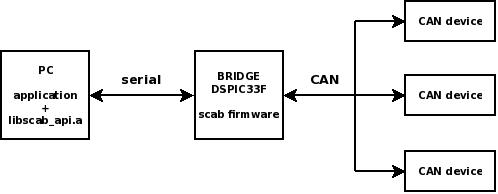
\includegraphics[scale=0.5]{./dia/scab_network/main.jpeg}
\caption{global view}
\label{global_view}
\end{figure}

\paragraph{}
Usually, PCs do not have the hardware interfaces required to communicate on a
CAN network. SCAB aims at adding CAN connectivity to PCs by bridging a serial
port. To do so, 2 softwares are provided:
\begin{itemize}
\item a firmware to be flashed on a DSPIC33F board,
\item a programming interface to be used by the client application.
\end{itemize}

\subsection{Availability}
\paragraph{}
The project source code is maintained in a GIT repository:
\begin{center}
https://github.com/texane/scab
\end{center}

\subsection{Dependencies}
\paragraph{}
The project depends on the following softwares:
\begin{itemize}
\item a working LINUX system with standard GNU tools,
\item MPLABX version 1.0 .
\end{itemize}
Note that WINDOWS and MACOSX are not yet supported.


\newpage
\section{Host programming interface}
\subsection{Compiling the library}
\subsection{Interface documentation}
\subsection{Example program}
\subsection{Limitations}


\newpage
\section{Device firmware}
\subsection{Limitations}


\newpage
\section{Host to device protocol}


\end{document}
